\chapter{Introduction}

Back at the end of {\it 1960’s} when the Internet was a rather small 
network, which was interconnecting major universities, governmental 
and military organizations, very little attention was devoted to 
security. Nowadays, when the Internet has become extremely 
sophisticated in structure, connecting billions of devices ranging 
from small IoT-type devices to humongous data centers, security has 
gained number one priority. In present days, a typical Intranet of 
an organization can include a number of geographically separated 
branch-office networks (for example, consider a factory that has 
many SCADA devices and a mission control center that is miles and 
miles away). Since these networks are geographically separated, connecting 
them becomes a necessity, and so is the security of these networks. 
This is when the layer-3 virtual private networks ({\it L3-VPN}) and layer-2 
virtual private LAN service ({\it L2-VPLS}) solutions become handy. 
Scalability, and resilience to various attacks, from man-in-the-middle 
to integrity violation attacks, to rather fundamental attacks on 
asymmetric algorithms (such as RSA, DSA, and their elliptic curve 
counterparts, Diffie-Hellman and Elliptic Curve DH, for example) 
using, for example, {\it Shor’s quantum computer algorithm} to factorize 
large numbers, and massive brute force attacks on hash algorithms 
should be considered thoroughly. With this in mind, in this work, we 
present different security solutions, which can be used to build secure 
L2 and L3 overlay networks. We present the limitations of each solution 
and identify how they can be avoided.

We start with background material on cryptography. 
Here we discuss various symmetric and asymmetric encryption algorithms, 
present the definition of hash functions, which are considered secure nowadays, 
and discuss several key agreement algorithms. To make the discussion 
complete we present the threat that quantum computers pose for such 
algorithms as RSA and DH, and discuss how post-quantum algorithms such 
as those that are based on the lattice can be used as an alternative to classical 
algorithms for encryption and signature constructions. Although not considered 
as part of the present work, future work can include the performance 
comparison of standardized RSA and DSA algorithms with the performance of 
lattice-based algorithms incorporated into for example Host Identity Protocol 
or even Transport Layer Security protocol. We then move on to a discussion of 
TLS, SSL, IPsec, HIP, and SSH protocols and how those can be used to achieve 
integrity and confidentiality of data transmitted over insecure channels. 
Afterward, we discuss the results we have obtained 
over several years. Here, we discuss our practical experience 
with scalable Host Identity Protocol-based L3-VPN and VPLS network which was 
built using the same protocol. We devote a separate section on 
hardware-accelerated versions of AES and SHA-256 algorithms. We conclude 
the results section with an analysis of the limitations of each solution 
and present the results for the various micro-benchmarking settings.

\section{Questions}

In this work, we ask several questions. These are not research questions, 
but rather practical questions that we try to answer to ourselves in order to 
understand the usability of Python-based security solution. Since our work 
focuses on the application of Host Identity Protocol (HIP) in VPN and VPLS 
settings we ask the following questions:

First, {\it what is the performance of the pure Python-based implementation of 
symmetric key encryption and decryption routines as well as hash methods and 
how do they compare to implementation, which uses special AES and SHA-256 CPU 
instructions.} Here our focus is on the micro benchmarking of two implementations 
of AES and SHA-256 hashing algorithms, identification of the bottlenecks and 
further recommendations for our prototype implementation of Host Identity Protocol 
based VPLS and L3-VPN.

Second, {\it what is the scalability of Host Identity Protocol based VPLS and how does 
it perform in emulated environments such as Mininet.} Here we seek the answer to 
the question of whether the HIP-VPLS is usable in environments close to real-life setups.

Third, {\it what is the performance of Python-based HIP-VPLS on real hardware}. By 
asking such questions we want to find the application niche of our security solution. In addition, 
we elaborate on the practical configuration of HIP-VPLS using a central controller.

The final question relates to {\it to the deployment of scalable L3-VPN 
based on Host Identity Protocol}. Here we focus on rather a different approach to building 
secure networks: we consider L3-VPN where nodes in different branch offices form separate 
broadcast and multicast domains, but still can communicate with each other (with the assistance of IPv4 or IPv6 
routing protocols). Here, we want to answer how to tackle the scalability issues of 
VPN network by adding hierarchy into the architecture.


\chapter{Background}

Since we are going to discuss the security protocols in this work, we begin 
this section with a shallow dive into cryptography basics. Here, we discuss 
symmetric and asymmetric cryptography algorithms, to make the description a 
little bit complete we show how the RSA algorithm works, discuss  
Diffie-Hellman (DH) and its Elliptic Curve counterpart. We should mention that the current 
understanding inside the cryptographic community is such that Shor’s algorithm and 
its quantum computer implementation theoretically 
can efficiently factorize big numbers and solve discrete logarithm problems without trouble. 
This algorithm, if powerful enough quantum computers will exist shortly, 
puts the RSA and DH algorithms - the major building blocks of modern security 
solutions - at risk of being cracked (once the modulus of the RSA algorithm factorized 
into prime components, the private key of the RSA 
the algorithm can be easily recovered). We will conclude this part of the background 
material with the discussion of {\bf post-quantum} computer public key encryption 
solution based on lattice (more specifically we will discuss Learning With Errors 
(LWE) the problem, which is at the heart of modern public key cryptography). 
We believe that, eventually, this type of cryptography will be 
the replacement for traditional RSA and DH algorithms, which rely on the hardness 
of factorization of the big numbers and discrete logarithm problems. In the epilogue of this 
section, we will put a few words on how lattice public key cryptography can be used, 
for example, together with Host Identity Protocol.

In the second part of the background material, we will review the basics of the Host 
Identity Protocol, Transport Layer Security Protocol, and Secure Shell Protocol, since 
these protocols are essential for understanding the secure tunneling protocols that we
discuss in this work.

We will finalize the discussion of the background material with a short overview of 
various L2, L3 and L4 tunneling solutions, including L2 802.1Q QinQ tunneling, 
L3 Multi-Protocol Label Switching (MPLS), L4 tunneling using TLS and SSH protocol.

\section{Cryptography basics}

Cryptography comes in many flavors: symmetric key cryptography 
(3DES, AES, Twofish, RC4) which, in turn, can be categorized into 
block cipher and stream cipher and asymmetric key cryptography 
(such as RSA, DSA, ECDSA). There are also key exchange protocols 
such as Diffie-Hellamn and Elliptic Cryptography DH for negotiation 
of common keys over insecure channels. Different algorithms applicable 
in different settings depending on requirements. Typically, as we will 
discuss later, symmetric key cryptography is used to protect 
data-plane traffic in networks, whereas, asymmetric-key cryptography is 
more applicable to the common key negotiation, authentication and 
identification purposes~\cite{Stinson:Cryptography}.

\subsection{Symmetric cryptography}

We start with the symmetric key cryptography. Common key and rather 
trivial operations such as permutations and substitutions are at the 
heart of any symmetric key cryptography algorithm. Although this type 
of cryptography is efficient because of the usage of efficient operations, 
it comes with a limitation though. In symmetric key cryptography, 
both sender and receiver need to share the same key, which complicates 
such important aspects as key distribution and revocation and so alone 
this encryption solution a very hard to use in modern cryptosystems. 
Typically, asymmetric key cryptography such as RSA or DH is used to derive session 
keys – TLS, HIP, and many other protocols follow this design idea.

Symmetric key cryptography comes in two different flavors: block and stream. 
For example, block cipher (such as AES, 3DES, Twofish~\cite{Stinson:Cryptography}) 
use blocks of data (typically, the size of the key is $128$, $192$, $256$ 
bits~\cite{Stinson:Cryptography}, and typical block size is $64$, or $128$ bits), and encrypts or 
decrypts one block at a time. There are different modes of operation, though, 
for block ciphers, examples are counter mode and cipher block chaining. 
The latter uses a so-called initialization vector to add extra randomness into the encryption 
process, and encryption of proceeding blocks depends on the output of the previous 
block. Modes of operations are important for security reasons. However, not all 
modes of operation are useful and secure. For example, Electronic Code Book (ECB), 
while achieving fast processing and parallelization, is considered insecure in 
many settings.

The other type of symmetric key algorithm is stream cipher. Here the encryption 
and decryption are performed on separate bits, one bit at a time. CR4 is an example 
of a stream cipher. Stream ciphers are extremely important in real-time processing, 
for example, Wi-Fi uses stream ciphers to encrypt the data plane traffic.

\subsection{Asymmetric cryptography}

Asymmetric key cryptography, in its simplest form, is brilliant in the age 
of computing. Guessing from the name that this type of cryptography uses different 
keys for encryption and decryption does not require deep thought. This property makes 
this group of algorithms suitable for various key distribution, revocation, and 
signature ideas. 

There is a magnitude of different asymmetric key security algorithms. 
RSA, DSA, and its Elliptic curve variant ECDSA are the pillars of modern 
security solutions. However, the flexibility of these schemes comes at an extra 
price of CPU cycles. All this makes these solutions inapplicable for securing 
data plane traffic, but only rather to secure control plane. In what follows, 
just to underpin the beauty of the math behind asymmetric key cryptography, 
we provide a description of the RSA algorithm.

In the RSA cryptosystem, the sender generates a pair of keys as follows: 
First, the sender chooses large enough two prime numbers $p$ and $q$. Next, 
the sender computes $n=pq$ and evaluates Euler’s phi function: $\phi(n)=(p-1)(q-1)$. 
This is the same as the number of numbers co-prime to $n$. The sender then selects at 
random encryption exponent $e$ such that $1<e<\phi(n)$ and also $e$ should be co-prime to $\phi(n)$.
Finally, the sender or the dealer computes the decryption exponent $d$, such that 
$ed \equiv 1\ mod\ \phi(n)$ using modular multiplicative inverse (for that purpose extended Euclidian 
algorithm can be used).

The public key is then $(n, e)$, and the private key is $(n, d)$. To encrypt the message $m$ 
the sender computes $c= m^e\ mod\ n$. The decryption is similar $m = c^d\ mod\ n$. The beauty is 
in Fermat’s little theorem, which states that $m^{\phi(n)}\ mod\ n \equiv 1\ mod\ n$. 
Now, $ed\ \equiv\ 1\ mod\ \phi(n)$, which means that 
$ed=k\phi(n)+1$, and so $m^{(ed)}\ mod\ n \equiv m^{(k\phi(n)+1)} mod\ n \equiv 1^k m\ mod\ n \equiv m\ mod\ n$. 

In practice, RSA requires random padding to protect against such attacks as chosen ciphertext 
attacks and making two identical plaintexts produce various ciphertexts. Padding also ensures that the 
message size is multiple of the encryption block-size. In practice, Optimal Asymmetric Encryption Padding (OAEP) 
scheme is used.

It is good to know that if the message is hashed and encrypted with the private key, the result is a 
form of digital signature since the sender cannot later deny that it was involved in the encryption 
process. A Digital Signature Algorithm (DSA) is another example of an asymmetric signature scheme and 
was specifically designed for that purpose. In turn, Elliptic Curves improve the performance of regular DSA 
algorithms.

Frankly speaking, one-way functions can be also used to construct signature schemes. 
For example, one can use one-time hash-based signatures to produce secure digital signatures. Nevertheless, 
the application of these types of signature algorithms is rather impractical and finds 
little application in real-life settings.

\subsection{Cryptographic hash functions}

Mathematically speaking, hash function is a special one-way function: For a given  
pre-image of an arbitrary size it produces an image or hash value of a fixed size, 
which is universally unique. Ideally, secure hash functions should guarantee 
that the result it produces is irreversible. That it is, it 
should be extremely hard to find a pre-image or original message, given the 
hash or the fingerprint. Secure hash functions should be also collision-resistant. 
In other words, it should be extremely hard, if not impossible at all, to 
find two different messages $m$ and $m’$ that will hash to the same value, i.e., 
$hash(m)=hash(m’)$.

Secure hash functions are important in modern cryptography. 
For example, they can serve as authentication tokens for messages transmitted over the 
wire (useful, for example, in detecting message manipulation during transmission), 
they also allow compressing the message before signing it with the digital signature 
algorithm, and, finally, they can be used to find the differences between the messages 
efficiently (useful in large file transfer operations). The application area is of 
course broader than just these few examples. 

Hash functions come in different flavors, but good ones should be computationally 
efficient and resistant to collisions. Today, hash functions such as MD2, MD4 and MD5 
considered broken, as there are works that showed successful attacks. Briefly speaking, 
researchers found collisions for these hash functions. Therefore, it is 
not recommended to use these hash functions in security applications. A more modern 
family of SHA hash functions also exists. For example, engineers recommend to use SHA-256, 
SHA-512 and recent SHA-3 in modern applications, as no successful attacks were registered for 
these types of hash functions.

Hash functions pave the road for such a notion as authentication tokens when combined with a 
secret key in a special way. Examples are Hash-based MAC (HMAC)~\cite{Stinson:Cryptography}, 
Parallelizable MAC (PMAC)~\cite{pmac}, Cipher-based MAC (CMAC) which is based on AES cipher. 
For instance, by sending an HMAC together with the original message one can make sure that 
the message will not be modified during the transmission. If, however, the message will 
be altered on the route to a recipient, this fact will be detected immediately during the 
verification process.

Hash functions are also useful in signatures. For example, one-time signatures use 
hash functions to construct a digital signature of a message. They are, however, impractical
as they require a considerable amount of storage and can be used only one time as the name implies. 
An interested reader can find more information about hash functions here~\cite{Stinson:Cryptography}.

\subsection{Key exchange protocols}

Finally, key exchange algorithms are also important in modern systems as they allow 
the negotiation of common keys over insecure channels. Of course, RSA can be used to deliver a session key
by encrypting it with the recipient's public key, but specially crafted key negotiation
algorithms exist in practice. Two bright examples are Diffie-Hellman (DH) and Elliptic Curve 
DH. Both DH and ECDH need to be authenticated in order to guarantee security.


\subsection{Post-quantum Lattice-based cryptography}

Shor's algorithm~\cite{shor}, implemented on a quantum computer, makes certain computational 
problems (such as factorization of large numbers and discrete logarithm problems) 
feasible in polynomial time. This shutters the security of the Internet, and 
so rigorous research was initiated to fill the gap. In what follows we discuss
certain hard mathematical problems on lattices and show the workings of the 
Learning With Errors (LWE) public key encryption scheme~\cite{regev}. In fact majority of 
NIST's candidates for post-quantum public key encryption algorithms are based 
on LWE.

A lattice is a mathematical structure that consists of integers in $n$ dimensions 
arranged in a structured lattice-like way. Mathematically, the lattice is defined as follows:
$$\Lambda({\bf B}) = \{{\bf Bx}, {\bf x} \in \mathbb{Z}^n \}$$ where ${\bf B}$ is a matrix of basis vectors
that generates the lattice. We should note that there exist a large number of basis vectors, some are {\it good}
some are {\it bad}.

A { \bf closest vector problem (CVP) } on lattices, which is considered NP-hard, and believed unsolvable even on 
quantum computers, can be defined as follows. Given a point $t \in \mathbb{R}^n$ and a lattice
$\Lambda({\bf B})$, the task is to find a closes point ${\bf Bx}$ on lattice: 

$$\min_{\forall {\bf x} \in \mathbb{Z}^n} \|{\bf Bx} - {\bf t}\|$$ 

In practice, the above problem is extremely hard to solve which makes lattice-based cryptography 
attractive to cryptographers.

From linear algebra we know that solving equation $\bf{Ax}=\bf{b}$ is simple using
Gaussian elimination. However, if a random noise is added to the equation $$\bf{Ax} + \bf{e} = \bf{b}$$ the 
problem is considered as hard as CVP on the lattice. Solving the above problem directly relates to 
solving the CVP problem on lattice if the parameters are selected carefully.

So, given a matrix $\bf{A} \sim U(\mathbb{Z}^{nxm}_q)$, vector $\bf{s} \sim U(\mathbb{Z}^{n}_q)$ and 
vector $\bf{e} \sim D_{\mathbb{Z}^{m}, \sigma}$ sampled from discrete (clipped) Gaussian distribution with parameter $\sigma$. We require that, the probability
$P[e < q/4]$ is high (\ie $99.99\%$) to ensure correct decryption of the message and to achieve the required 
level of security. We can define matrix ${\bf A}$, secret key ${\bf s}$ and noise vector ${\bf e}$ as follows:

\begin{equation}
 {\bf A}=\begin{bmatrix}
 a_{11}       & a_{12} & a_{13} & \dots & a_{1n} \\
 a_{21}       & a_{22} & a_{23} & \dots & a_{2n} \\
 \hdotsfor{5} \\
 a_{m1}       & a_{m2} & a_{m3} & \dots & a_{mn}
    \end{bmatrix}
\end{equation}

\begin{equation}
 {\bf s}=\begin{bmatrix}
 s_{1} \\
 s_{2} \\
 \dots \\
 s_{n} 
    \end{bmatrix}
\end{equation}

\begin{equation}
 {\bf e}=\begin{bmatrix}
 e_{1} \\
 e_{2} \\
 \dots \\
 e_{m} 
    \end{bmatrix}
\end{equation}

Once the parameters are generated, we can compute ${\bf As}+{\bf e} = {\bf b}$. Then, the public 
key is $({\bf A, b})$ and the private key is ${\bf s}$. Deriving ${\bf s}$ from ${\bf b}$ is a hard 
task at hand.

To encrypt the message $\mu \in \{0, 1\}$, we choose ${\bf r} \sim U(\{0, 1\}^m)$. Then we compute ${\bf u}={\bf rA}$ and 
$v={\bf rb}+\lfloor q/2 \rceil \mu$. The ciphertext is $({\bf u}, v)$. To decrypt the message we can 
compute $v - \bf{u s}$: if the result is less than $q/4$ output $0$, otherwise, if the result
is larger than $q/4$ output $1$. For decryption to work correctly, we require that the parameter $\sigma = q/(16m)$. 

The major disadvantage of lattice-based cryptography is the size of the keys and actual ciphertext. For example,
the security of LWE depends on two parameters $n$ and $q$. By choosing $n=512$ and $q=2^{16}$, the size of ciphertext
for a message of $k=256$ bits long (for example, this is the size of the key for AES-256 symmetric algorithm), 
will be $O(k \cdot n \cdot \log q) \approx 256 \cdot 16 \cdot 512$ bits or roughly whooping 
$256$ KB. All in all the security does not come for free. Of course, there are way much practical implementations
of LWE-based encryption algorithms, for example, the reader can take a look at Kyber~\cite{nist:kyber} which has a practical 
implementation in the TLS library.

\section{Security protocols}

Equipped with a basic understanding of cryptography we will now dive into a discussion of some 
of the well-known security protocols, including IPSec, HIP, TLS, and SSH. All these protocols
make a solid basis for secure internetworking.

\subsection{Host Identity Protocol (HIP)}

Internet was designed initially so that the Internet Protocol (IP) address has a dual role: it 
is the locator, so that the routers can find the recipient of a message, and it is an identifier 
so that the upper layer protocols (such as TCP and UDP) can make bindings (for example, transport 
layer sockets use IP addresses and ports to make connections). This becomes a problem when a networked 
device roams from one network to another, and so the IP address changes, leading to failures in 
upper-layer connections. The other problem is the establishment of an authenticated channel between 
the communicating parties. In practice, when making connections, the long-term identities of the parties 
are not verified. Of course, solutions such as SSL can readily solve the problem at hand. However, SSL 
is suitable only for TCP connections, and most of the time, practical use cases include only secure web 
surfing and the establishment of VPN tunnels. Host Identity Protocol, on the other hand, is more flexible: 
it allows peers to create authenticated secure channels on the network layer, so all upper-layer protocols 
can benefit from such channels. More on the protocol can be found in~\cite{gurtov:hip}.

HIP relies on the 4-way handshake to establish an authenticated session. During the handshake, the 
peers authenticate each other using long-term public keys and derive session keys using Diffie-Hellman 
or Elliptic Curve (EC) Diffie-Hellman algorithms. To combat the denial-of-service attacks, HIP also 
introduces computational puzzles. 

HIP uses a truncated hash of the public key as an identifier in the form of an IPv6 address and 
exposes this identifier to the upper layer protocols so that applications can make regular 
connections (for example, applications can open regular TCP or UDP socket connections). At the 
same time, HIP uses regular IP addresses (both IPv4 and IPv6 are supported) for routing purposes. 
Thus, when the attachment of a host changes (and so does the IP address used for routing purposes), 
the identifier, which is exposed to the applications, stays the same. HIP uses a particular 
signaling routine to notify the corresponding peer about the locator change. More information 
about HIP can be found in RFC 7401~\cite{rfc7401}. 

\subsection{Transport Layer Security (TLS)}
Secure socket layer (SSL)~\cite{ssl} and Transport Layer Security (TLS)~\cite{tls} are an application 
layer solutions to secure TCP connections. SSL was standardized in RFC 6101. 
TLS was standardized in RFC 5246. And was designed to prevent eavesdropping, 
man-in-the-middle attacks, tampering, and message forgery. In SSL communicating 
hosts can authenticate each other with the help of longer-term identities - public key certificates.
SSL is great for building VPN tunnels and protecting upper-layer protocols such as HTTP.


\subsection{Secure Shell Protocol (SSH)}

Secure Shell protocol (SSH) is the application layer protocol that provides an encrypted channel 
for insecure networks. SSH was originally designed to provide secure remote command-line, login, 
and command execution. But in fact, any network service can be secured with SSH. Moreover, SSH 
provides a means for creating VPN tunnels between spatially separated networks: SSH is a great 
protocol for forwarding local traffic through remote servers. 

\section{L2, L3 and L4 tunneling}

Virtual Private LAN Services (or VPLS), L3-VPNs, and L4 tunneling are pretty standard nowadays. 
Companies build security solutions to provide Layer-2 and Layer-3 services for branch offices: 
VPLS are typically built as overlays on top of Layer-3 (IP) and are Ethernet over IP type 
overlays, whereas L3-VPNs are IP-in-IP tunneling solutions.

In VPLS, when a frame arrives at VPLS provider equipment (PE), it is encapsulated 
into an IP packet and is sent out to all other VPLS network elements comprising emulated LAN. 
Security of such overlays is important for obvious reasons: customers do not want their corporate 
traffic to be sniffed and analyzed. In L3-VPN networks, on the other hand, the networks form different 
broadcast domains, and so when an IPv4 or IPv6 packet arrives at the VPN box, it is encapsulated in another 
IP packet and sent out using the backbone network. In this work, we built such secure overlays with 
Host Identity Protocol. 

In this section, however, we will briefly review some of the widely used solutions 
for building L2, L3 and L4 overlays.

\subsection{Virtual Private LAN Services (VPLS) solutions}

\eat{
Virtual Private LAN Services (VPLS) are pretty common nowadays. 
}
In this section we will cover 
to standard ways to build VPLS networks (using, for example, 802.1q QinQ tunneling and MPLS).

\subsubsection{QinQ tunneling}

When the path from one network to the other, such as branch office to head office,
traverses only layer-2 switches (\ie no IP routing is involved), the VPLS can be organized 
with the help of 802.1Q protocol~\cite{snr}. Broadly, speaking this is not a protocol as such, but rather 
VLAN tag-based switching. Thus, on the ingress point, an additional 802.1q service provider SP-VLAN tag 
is inserted in the L2 header of an Ethernet frame. Later, the forwarding decisions are 
made using this SP-VLAN tag. On the egress point, the SP-VLAN tag is removed and the original 
Ethernet frame is forwarded to the recipient based on the destination MAC address 
and, if exists, on the inner C-VLAN tag. 

It should be noted that the configuration of forwarding is a manual step.
Also, QinQ does not provide additional mechanisms to secure the customer's traffic,
thus limiting the application domain of this solution.

\subsubsection{MPLS tunneling}

Multi-protocol label switching is a standard protocol for forwarding any traffic type.
It is a layer $2.5$ solution that sits between the data link layer and the network layer.

In MPLS the packets are forwarded not using MAC or IP addresses, but 
rather using labels, which are distributed by control protocol. Thus, when a frame 
arrives at the router the current label is popped, the new label is added and the frame is
forwarded to the next hop router. The process continues until the frame reaches the 
destination network where it is routed based on the original identifiers (IP addresses or MAC addresses).
Obviously, MPLS has label distribution protocol and label switching components.
MPLS is an ideal solution to create overlays (\ie L2 and L3 VPNs).

\subsection{Virtual Private Network (L3-VPN) security solutions}

The major drawback of QinQ and MPLS is that they do not offer encryption and 
authentication of traffic out-of-the box. Therefore, additional steps needs to be taken to protect end-to-end
traffic. In this section we will review PPTP, SSL-based VPNs, L2TP and IPsec tunnels.

\subsubsection{Multipoint to single point VPN}

Multipoint to single-head VPN is a standard way of organizing a VPN network
for an organization that has a single head office and multiple branch offices.
In this setup, multiple branch offices are connected to a head end. 
We show such a setup in Figure~\ref{fig:head-vpn}.

\begin{figure}[ht!]
    \centering
    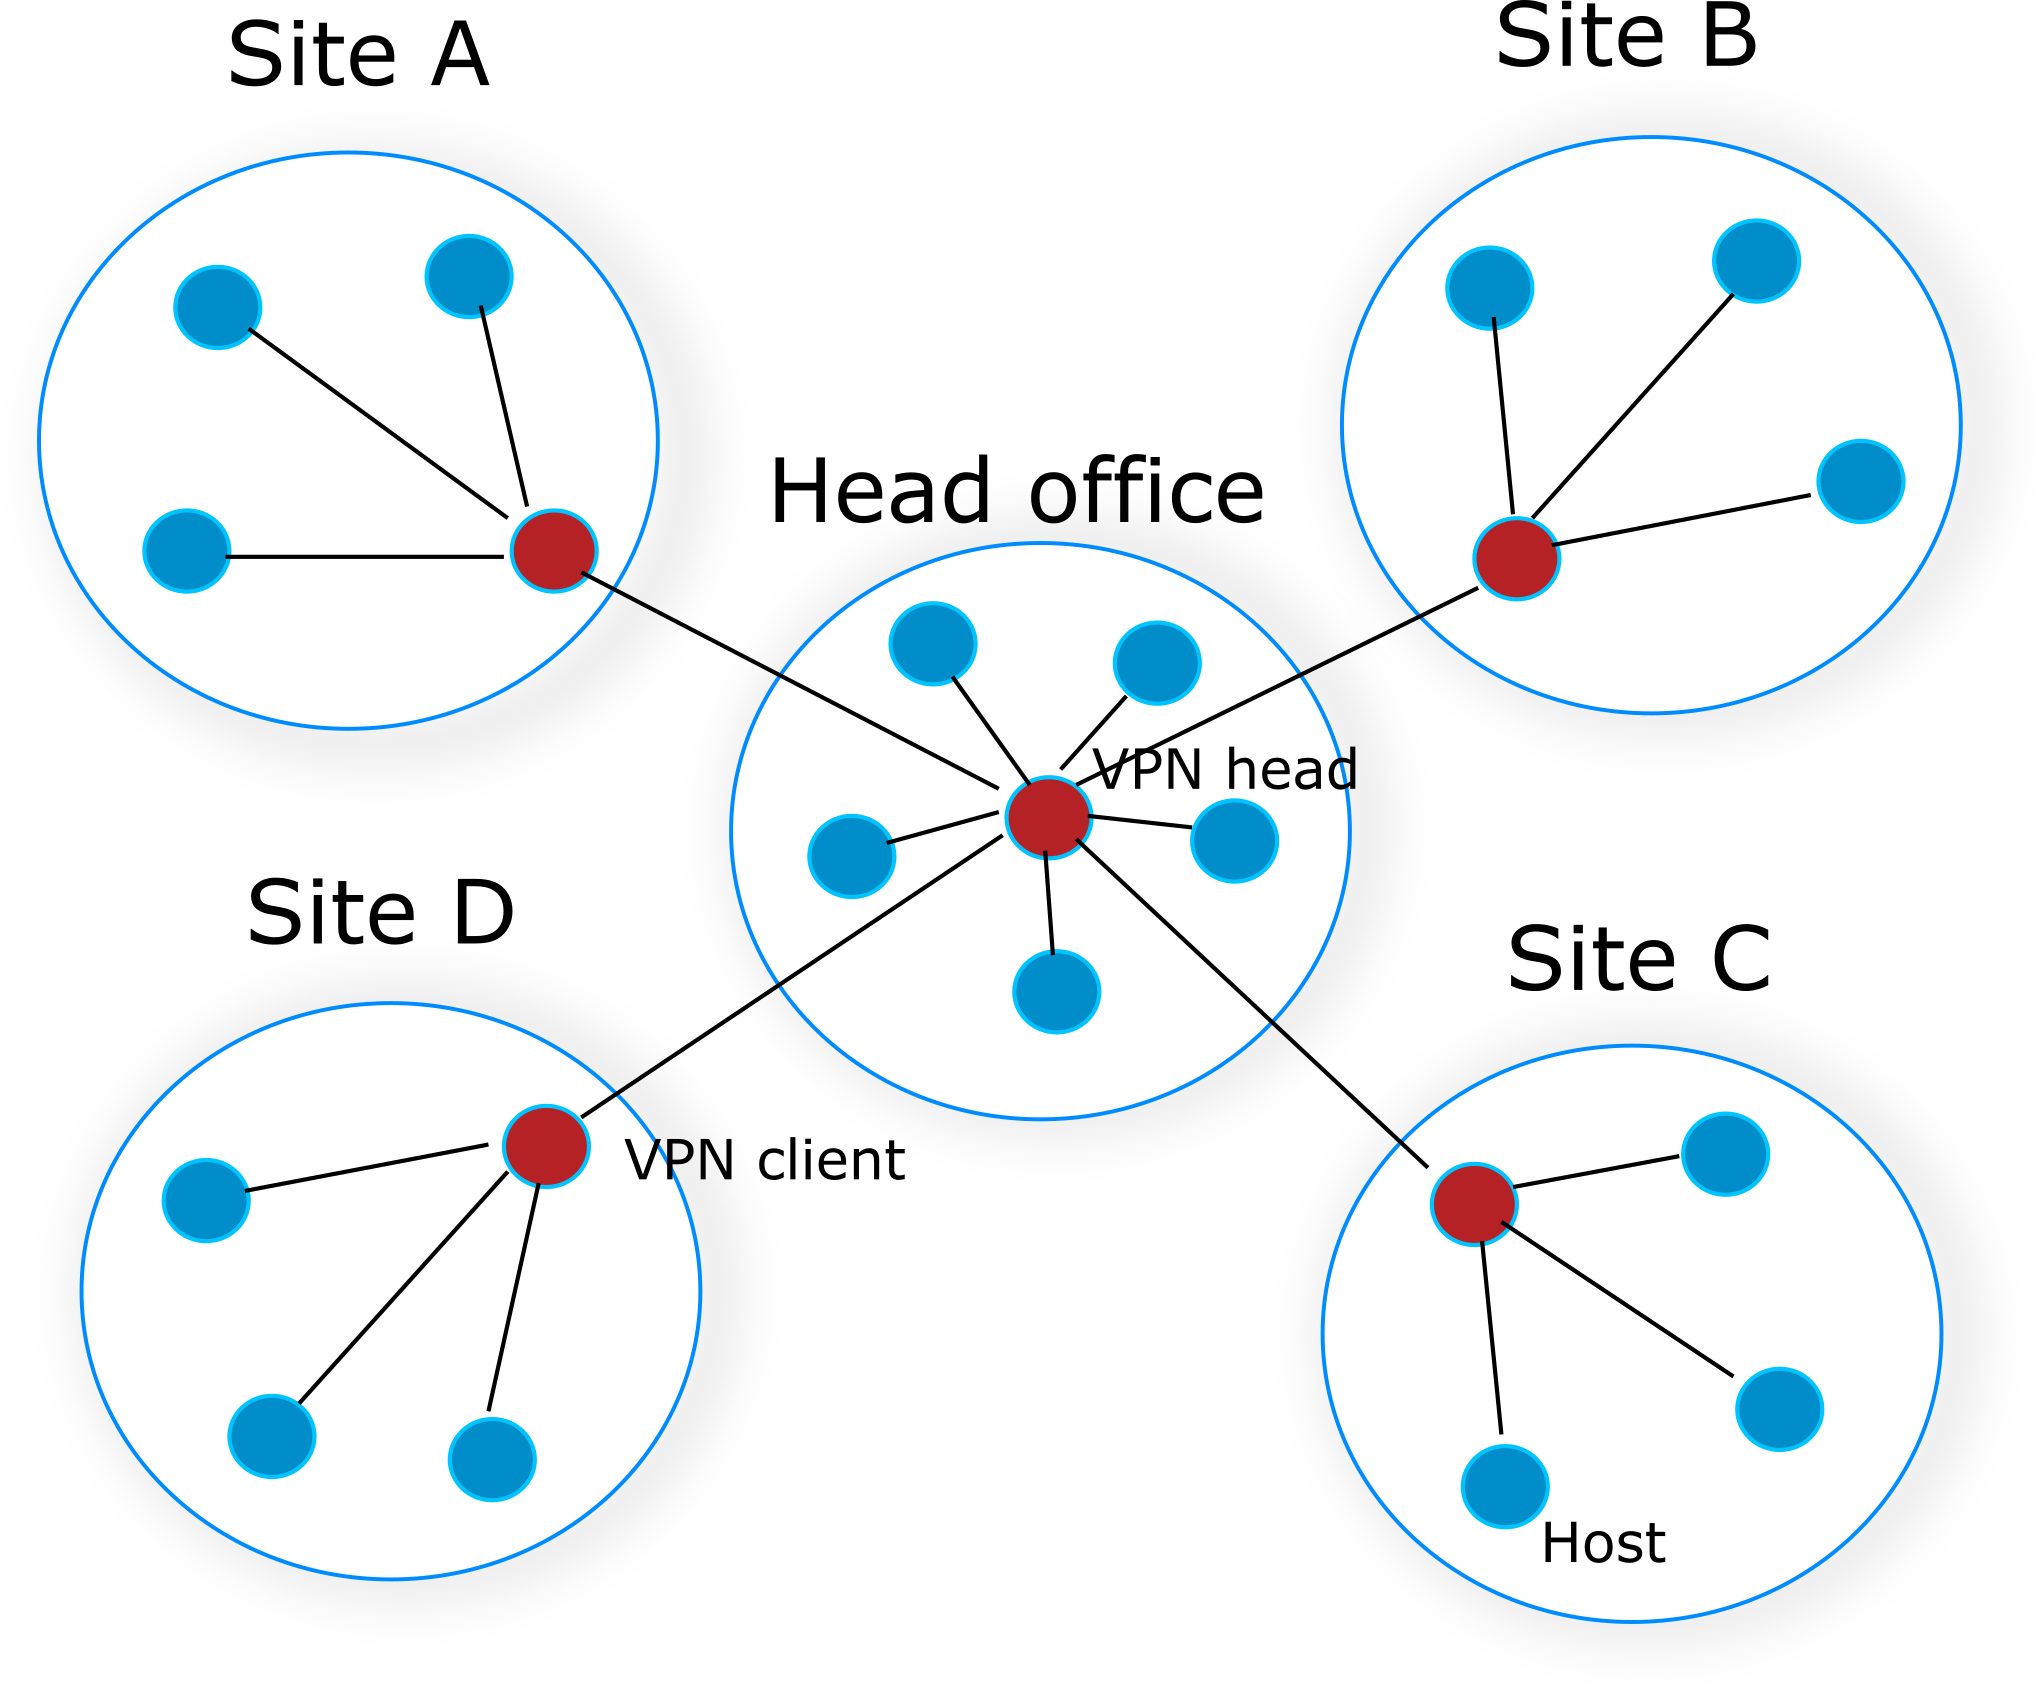
\includegraphics[width=0.9\textwidth]{graphics/vpn-central.png}
    \caption{Typical arrangement of the VPN}
    \label{fig:head-vpn}
\end{figure}

There are several protocols available for such an arrangement. Examples are:
(i) Point-to-Point Tunneling Protocol (PPTP)~\cite{tcpip}; (ii) Generic Routing Encapsulation (GRE)~\cite{tcpip}; 
(iii) SSL-based Secure Socket Tunneling Protocol (SSTP); (iv) Layer 2 Tunneling Protocol (L2TP)~\cite{tcpip}, 
which is an older protocol that can be combined with IPSec for encryption;
(v) Internet Protocol Security (IPSec).

GRE on its own does not provide security and can be used together with IPsec to secure 
the traffic. PPTP, in turn, does not provide strong security out of the box. PPTP uses 
weak Microsoft Point-to-Point Encryption (MPPE), which is considered insecure. PPTP combines 
GRE and PPP protocols under a single umbrella. It is the PPP protocol~\cite{tcpip}
that provides such services as authentication (using MS-CHAPv2, PAP or strong EAP protocol) 
and link configuration (\ie using Link Control Protocol (LCP)). Overall, it is not recommended
to use PPTP in modern VPN setups. L2TP with IPSec AES-256 encryption is more secure alternative.

SSTP protocol is built on top of existing SSL. It allows tunneling user traffic over protected 
channel, and yet the traffic looks like normal HTTPS traffic to service providers.
We have, ourselves, created a similar in spirit L3-VPN solution that is based on SSL~\cite{ssl:vpn}.
The solution operates on a standard HTTPS port. However, our idea is to tunnel 
all traffic from VPN-agnostic hosts through the off-the-path black box that encrypts 
all traffic and sends encapsulated in TCP and SSL
packets to the L3-VPN head server. The solution that we have created is a simple script 
that allows us to set up such an arrangement with no hassle. One drawback is that it 
uses TCP for transport: sending over a reliable TCP channel and over well known HTTPS port
is good for bypassing the traffic filters, but reduces the performance especially if
the channel has a large latency and error rate. 

IPSec~\cite{tcpip} comes in two variations: Authentication Header (AH) and Encapsulating Security Payload (ESP).
The first does not encrypt the data-plane traffic but rather adds HMAC to the packet. The second one, in
addition to authentication, adds encryption of the payload. IPSec, when combined with the key exchange 
protocols, such as Internet Key Exchange (IKE)~\cite{rfc4306}, can be used to create secure tunnels between the sites.

\subsubsection{SSH tunneling}

SSH, despite that it was invented for remote access to Linux-like boxes, can be used 
to tunnel local traffic to remote machine and remote traffic to local machine~\cite{ssh:tunneling}. Thus, it can be used to create
layer-4 tunnels. For example, the following command will tunnel all local traffic from
port 4443 to remote web-server {\it youtube.com} on port 443:

\begin{verbatim}
ssh -L 192.168.1.1:4443:youtube.com:443 user@strangebit.io
\end{verbatim}

In this example, when the client types \url{https://192.168.1.1:4443/} in the browser window,
the traffic will be forwarded to the remote {\bf youtube} server through the SSH server \url{strangebit.io}.

There is also a possibility to perform reverse tunneling, \ie one can expose the local service to the world.
For example, suppose you have a precious MySQL resource in your local network running on host \url{192.168.1.45} 
on port $3306$, then you can expose the service to the world using the following command:

\begin{verbatim}
ssh -R 0.0.0.0:3306:192.168.1.45:3306 user@strangebit.io
\end{verbatim}

This way various tunneling setups can be organized making SSH an attractive secure tunneling 
solution.

\chapter{Results}

In this chapter, we are going to present the results that we have obtained 
throughout the several years that we have spent building various systems. We start 
with the results for the cryptographic library which we have implemented to 
boost the performance of AES and HMAC algorithms on Intel CPUs. We then 
present the results for complete HIP-VPLS architecture and present the 
looking of the web interface which was used to configure the HIP switches.
Finally, we present the design and implementation of the hierarchical L3-VPN
in the Mininet emulator.  

\section{Hardware-enabled symmetric cryptography}

Part of the work that we have done was related to porting parts of the code to pure C 
and special Intel CPU instructions. In this section, we will describe our achievements 
in this direction. 

For the benchmarking, we have selected three implementations. The first one was pure 
Python based. For that purpose, we have used PyCryptodome library. The second implementation
was a Python wrapper to the C library that used special Intel CPU instructions to boost 
the AES and SHA-based HMAC operations. The third implementation was pure C library 
which was using Intel NI instructions. The results for AES-256 and HMAC operations 
for varying block sizes are shown in Figure~\ref{fig:aes} 
and in Figure~\ref{fig:hmac}. The plots show the average 
running time in microseconds with the $95\%$ confidence intervals. 

\begin{figure}[!ht]
    \centering
    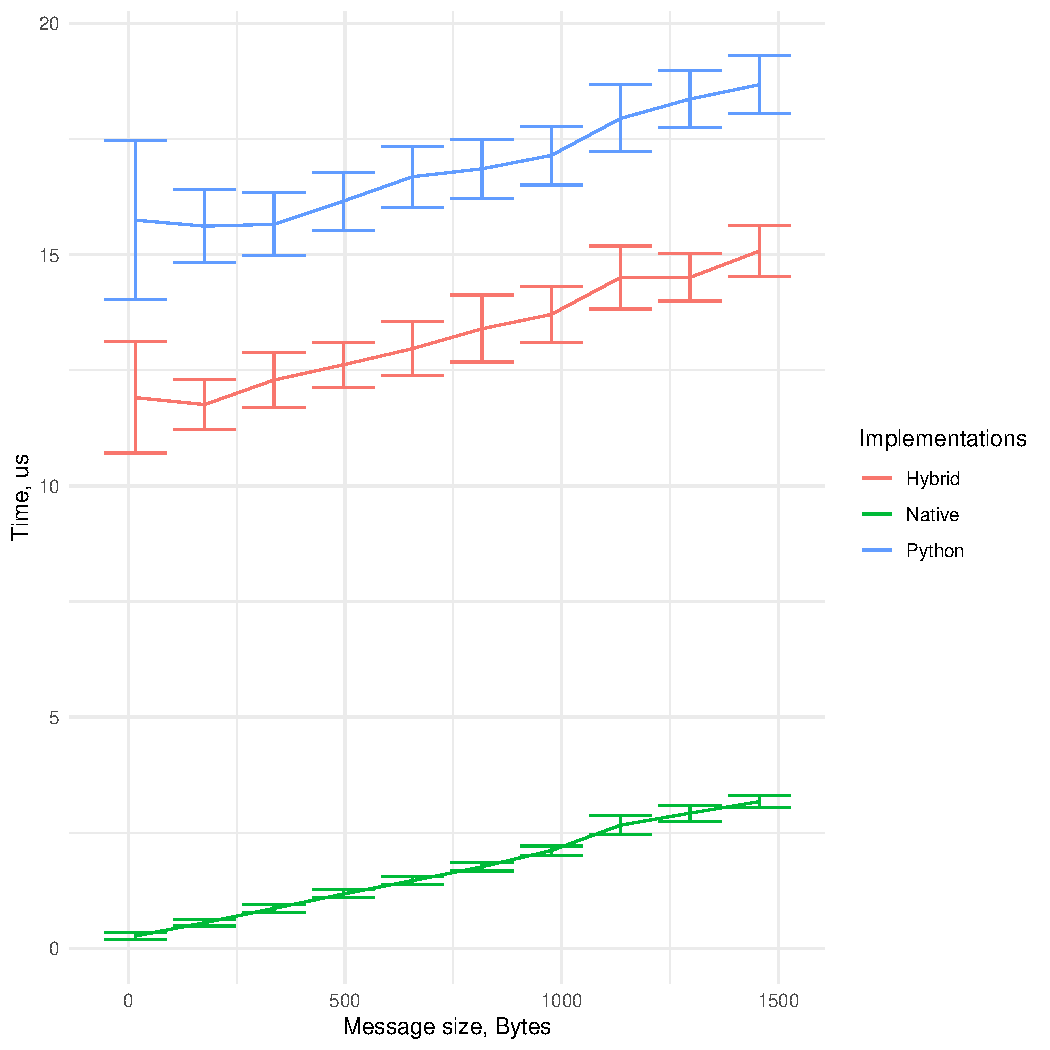
\includegraphics[width=0.9\textwidth]{graphics/crypto/aes.pdf}
    \caption{AES-256 encryption (microseconds)}
    \label{fig:aes}
\end{figure}

\begin{figure}[!ht]
    \centering
    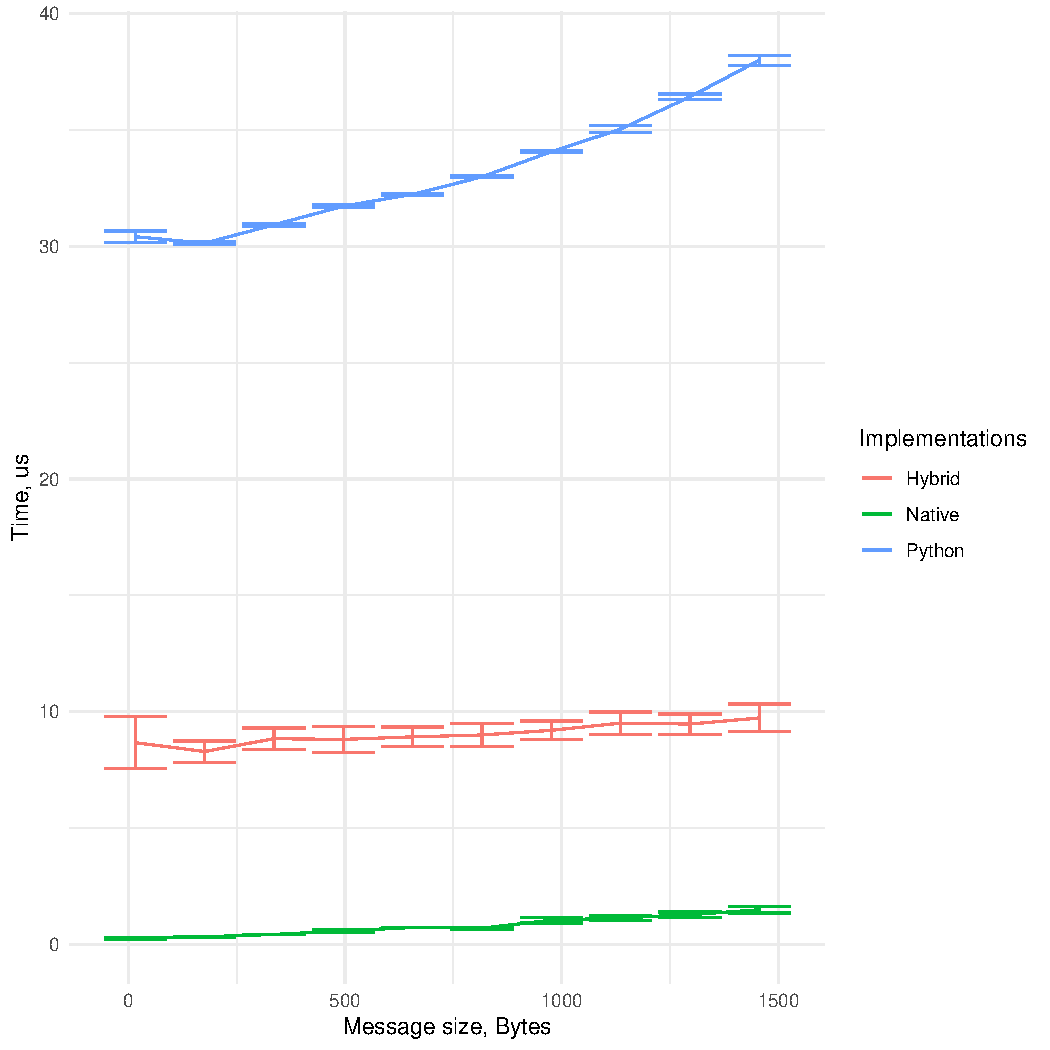
\includegraphics[width=0.9\textwidth]{graphics/crypto/hmac.pdf}
    \caption{HMAC calculation (microseconds)}
    \label{fig:hmac}
\end{figure}


What does this mean to HIP-VPLS performance? For a standard packet of size $1500$ 
bytes we have compared the performance (combined HMAC and AES-256) and it turned 
out, on one hand, that the implementation of cryptography in pure C with special CPU instructions was 
$12.1$ faster than pure Python implementation. On the other hand, Python implementation with bindings
to C library demonstrated performance which was $2.3$ times faster. By making back of the envelop calculations
we predict that Python implementation can achieve roughly $461$ Mbit/s in upload and download directions
cumulatively. However, in practice, given other operations with packets, we did not get this result 
in our experiments (more about the performance of HIP-VPLS on real hardware can be found in the proceeding 
chapter). For the plain C implementation with AES and SHA instructions, the performance will be 
better and constitute an astonishing $2.5$ Gbit/s. If someone needs to run the code in production
the entire code needs to be rewritten in plain C or Rust programming language for adequate performance.

\section{Host Identity Protocol based VPLS}

Virtual Private LAN Services (VPLS) provide means for building Layer 2 communication 
on top of existing IP networks. As we have mentioned already, VPLS can be built using various approaches. However, 
when building a production-grade VPLS solution one needs to have a clear picture of 
how such aspects as security and scalability will be solved.

In what follows, we will demonstrate how to build the VPLS using Host Identity Protocol (HIP). 
Our initial goal was not to build a production-grade implementation of HIP switches. Instead, 
at first, we were only interested in demonstrating proof of a concept solution in 
Mininet~\cite{mininet} – a framework for emulating L2 and L3 networks. It is worth mentioning that the code 
we have produced can be also deployed (under certain conditions; for example, our HIP implementation 
does not feature the NAT traversal mechanisms) on the real hardware in the Internet. We are going to demonstrate 
a working prototype in the later part of this work (here we assume that the public IPs are not from private 
range). All our prototypes use Python-based HIP~\cite{pyhip} as the bases.

While building HIP switches (the switches that are deployed at the border of a network and are responsible 
for setting up security associations and pseudowires) we came across several challenges. 
First, to avoid loops the underlying network needs to support 
the IEEE 802.1D protocol (or its modification - this really depends on the version of the protocol 
supported by the switches). This problem was initially addressed in the relevant IETF draft. 
For the sake of brevity, we note that if LAN implements 802.1D STP protocol there will be no loops in the 
HIP-VPLS instance. Second, there were certain issues with MTU and the inability of the Linux kernel to deliver IP 
packets when those are fragmented in user space and injected into the network stack using raw 
sockets. And finally, it took us some time to repackage the existing implementation of HIP protocol 
as a library, so that it would be agnostic about low-level networking (such as raw sockets, etc.). 
In the proceeding paragraphs, we will demonstrate the usage of HIP-based VPLS using loop-free L2 topology.

The logical network diagram of our Mininet prototype is shown in the Figure~\ref{fig:mininet}.

\begin{figure}[h!]
    \centering
    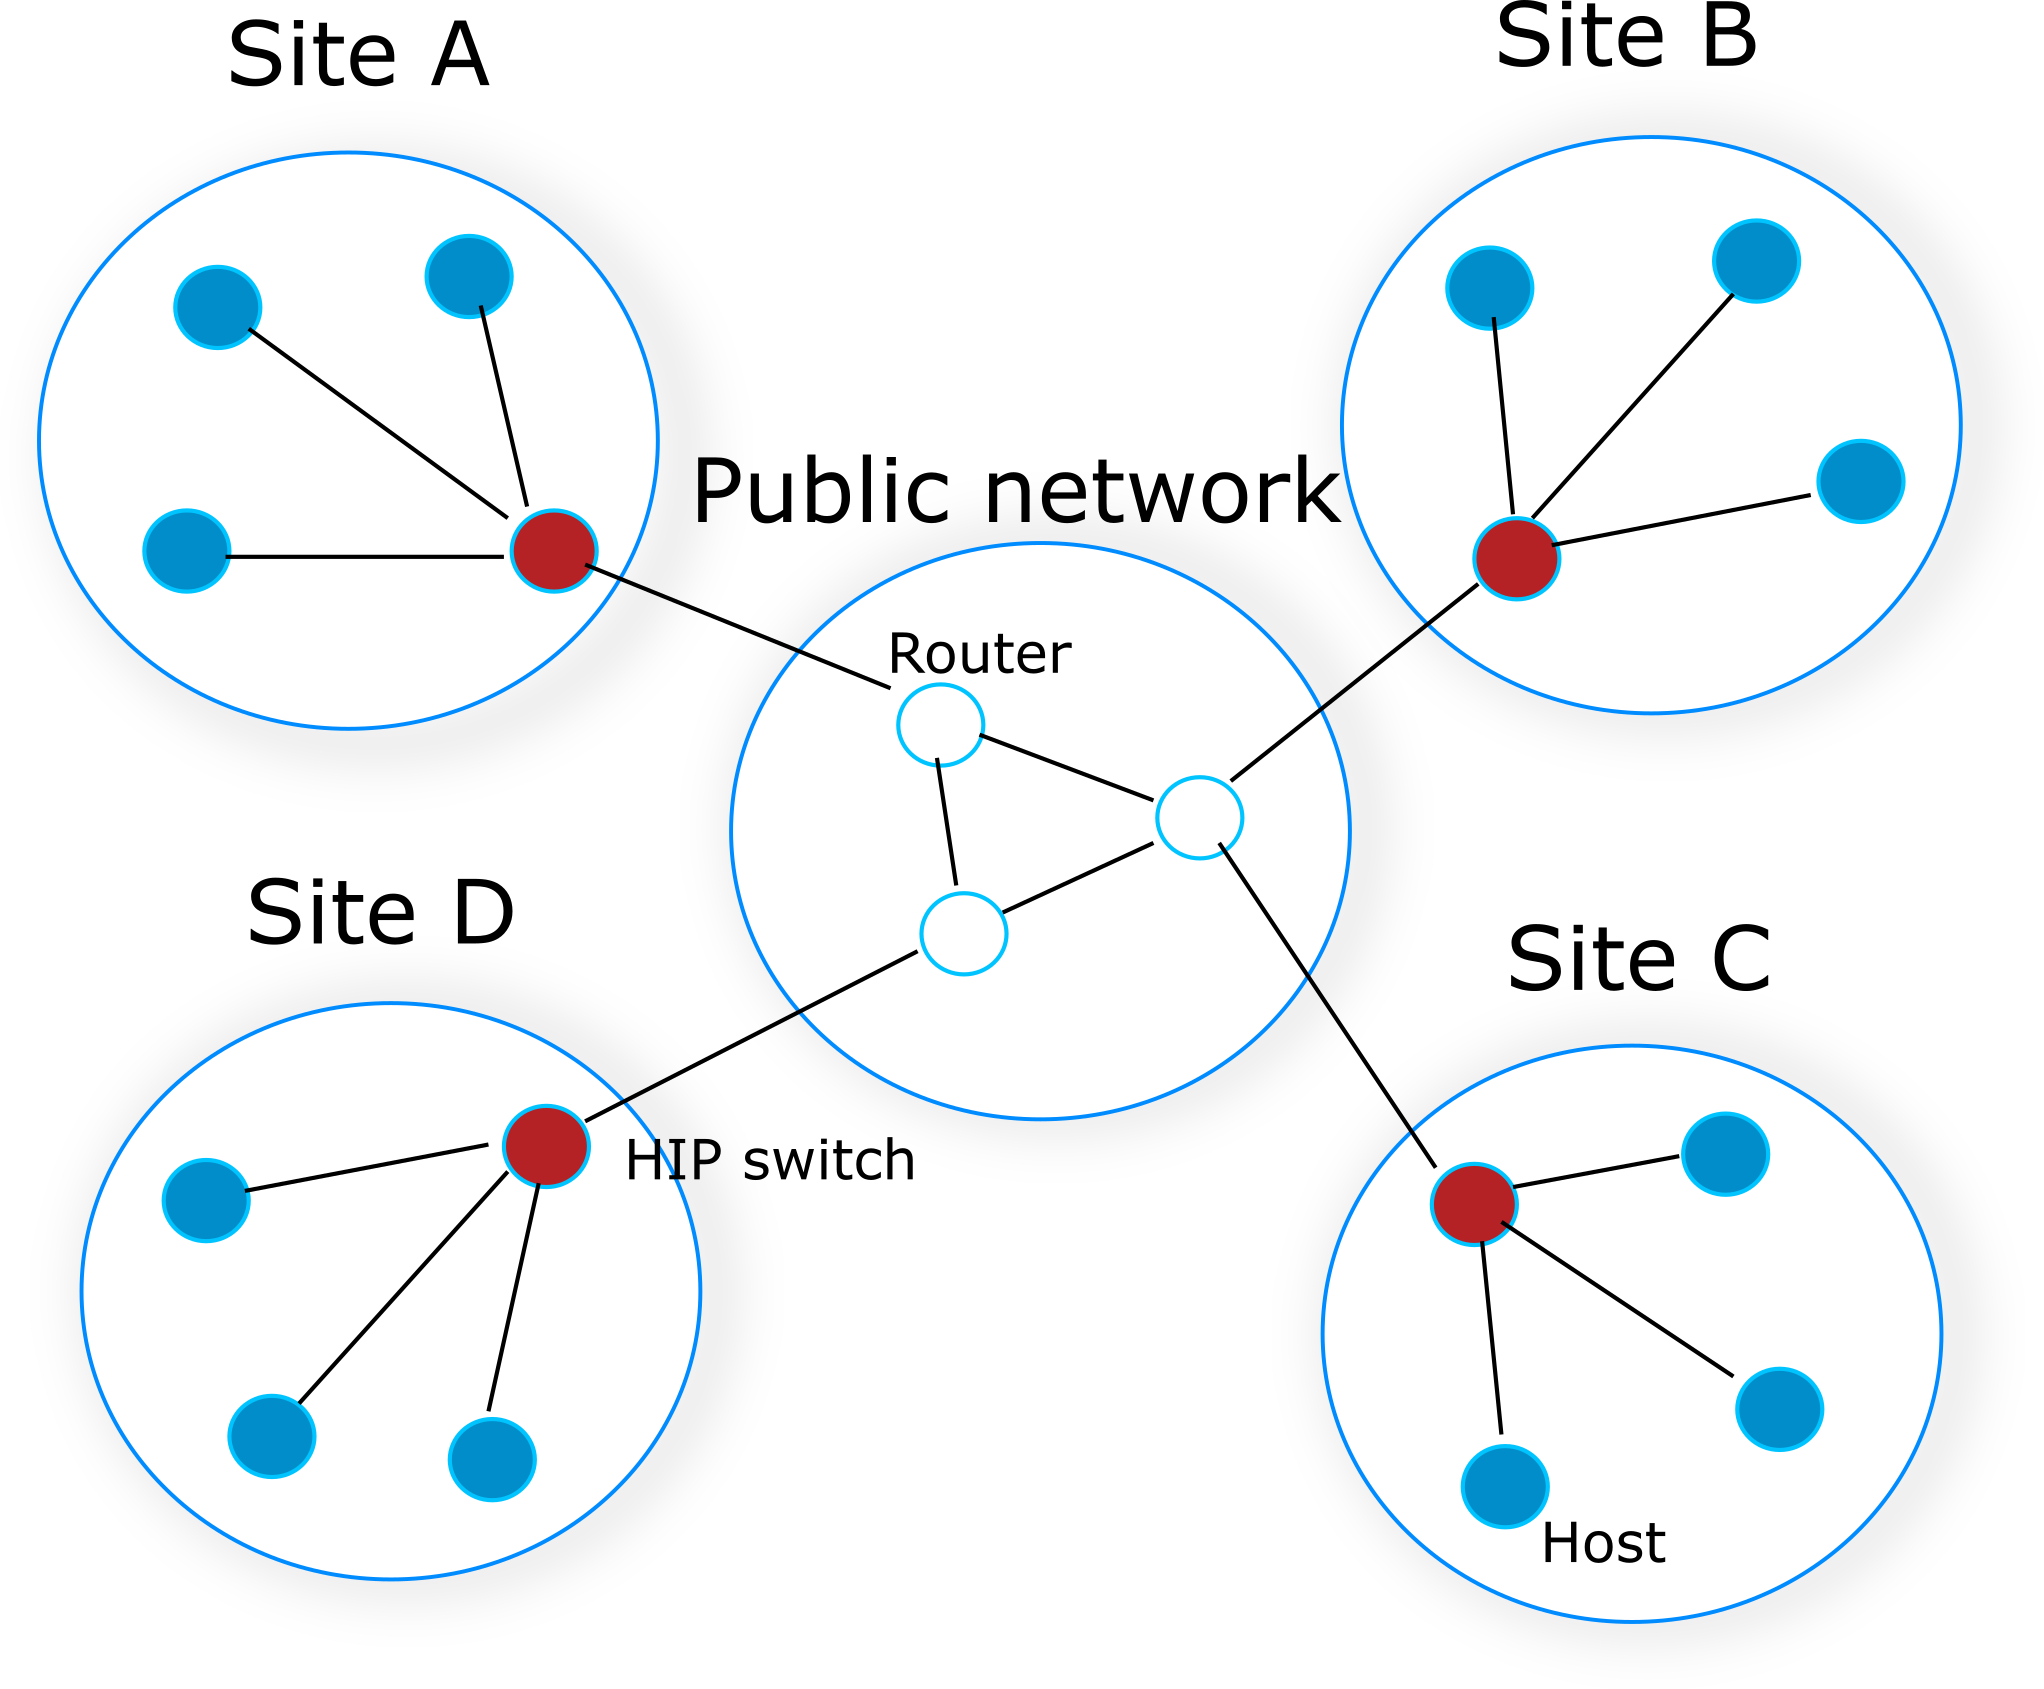
\includegraphics[width=0.7\textwidth]{graphics/mininet.png}
    \caption{HIP-VPLS logical diagram (Mininet deployment)}
    \label{fig:mininet}
\end{figure}

Our HIP-VPLS implemnetation~\cite{hip-vpls:mininet} in Mininet was using static configuration, meaning that 
HIP-VPLS mesh, resolver and firewall rules were configured prior to deployment 
of the overlay network and remained unchanged throughout the experiments. An interested reader
can take a look at~\cite{hip-vpls:mininet} for precise steps that are required to 
deploy the HIP-VPLS in the Mininet environment.

Overall, HIP-VPLS works as follows: (i) The daemon constantly listens for packets on private interface 
and public interface; (ii) if the frame, which arrives on the private interface, is broadcast or multicast 
daemon chooses all HIP-VPLS peers in mesh to send the packet; 
(iii) if the frame is unicast and HIP security association exists for the destination daemon 
sends the packet to the selected HIP switch; (iv) if no security association exists HIP switch triggers 
HIP base exchange to negotiate secret keys and to establish security association; (v) If the 
IPSec packet arrives on the public interface, first HMAC is verified, and if it is valid the packet 
is decrypted; the original Ethernet frame is then reinjected into the private interface and 
regular destination MAC-based and VLAN-based forwarding is performed to deliver the frame to the recipient. 

Our HIP switch also implements the MAC learning and aging functionality: whenever a frame arrives 
on the public interface the HIP-switch notes the source MAC address 
and adds it to the local database. Later, when a unicast frame arrives on the private interface, 
it looks up the destination MAC address and chooses the corresponding HIP association and pseudowire to send
the frame encapsulated into an IPSec packet to the recipient. 


\begin{figure}[h!]
    \centering
    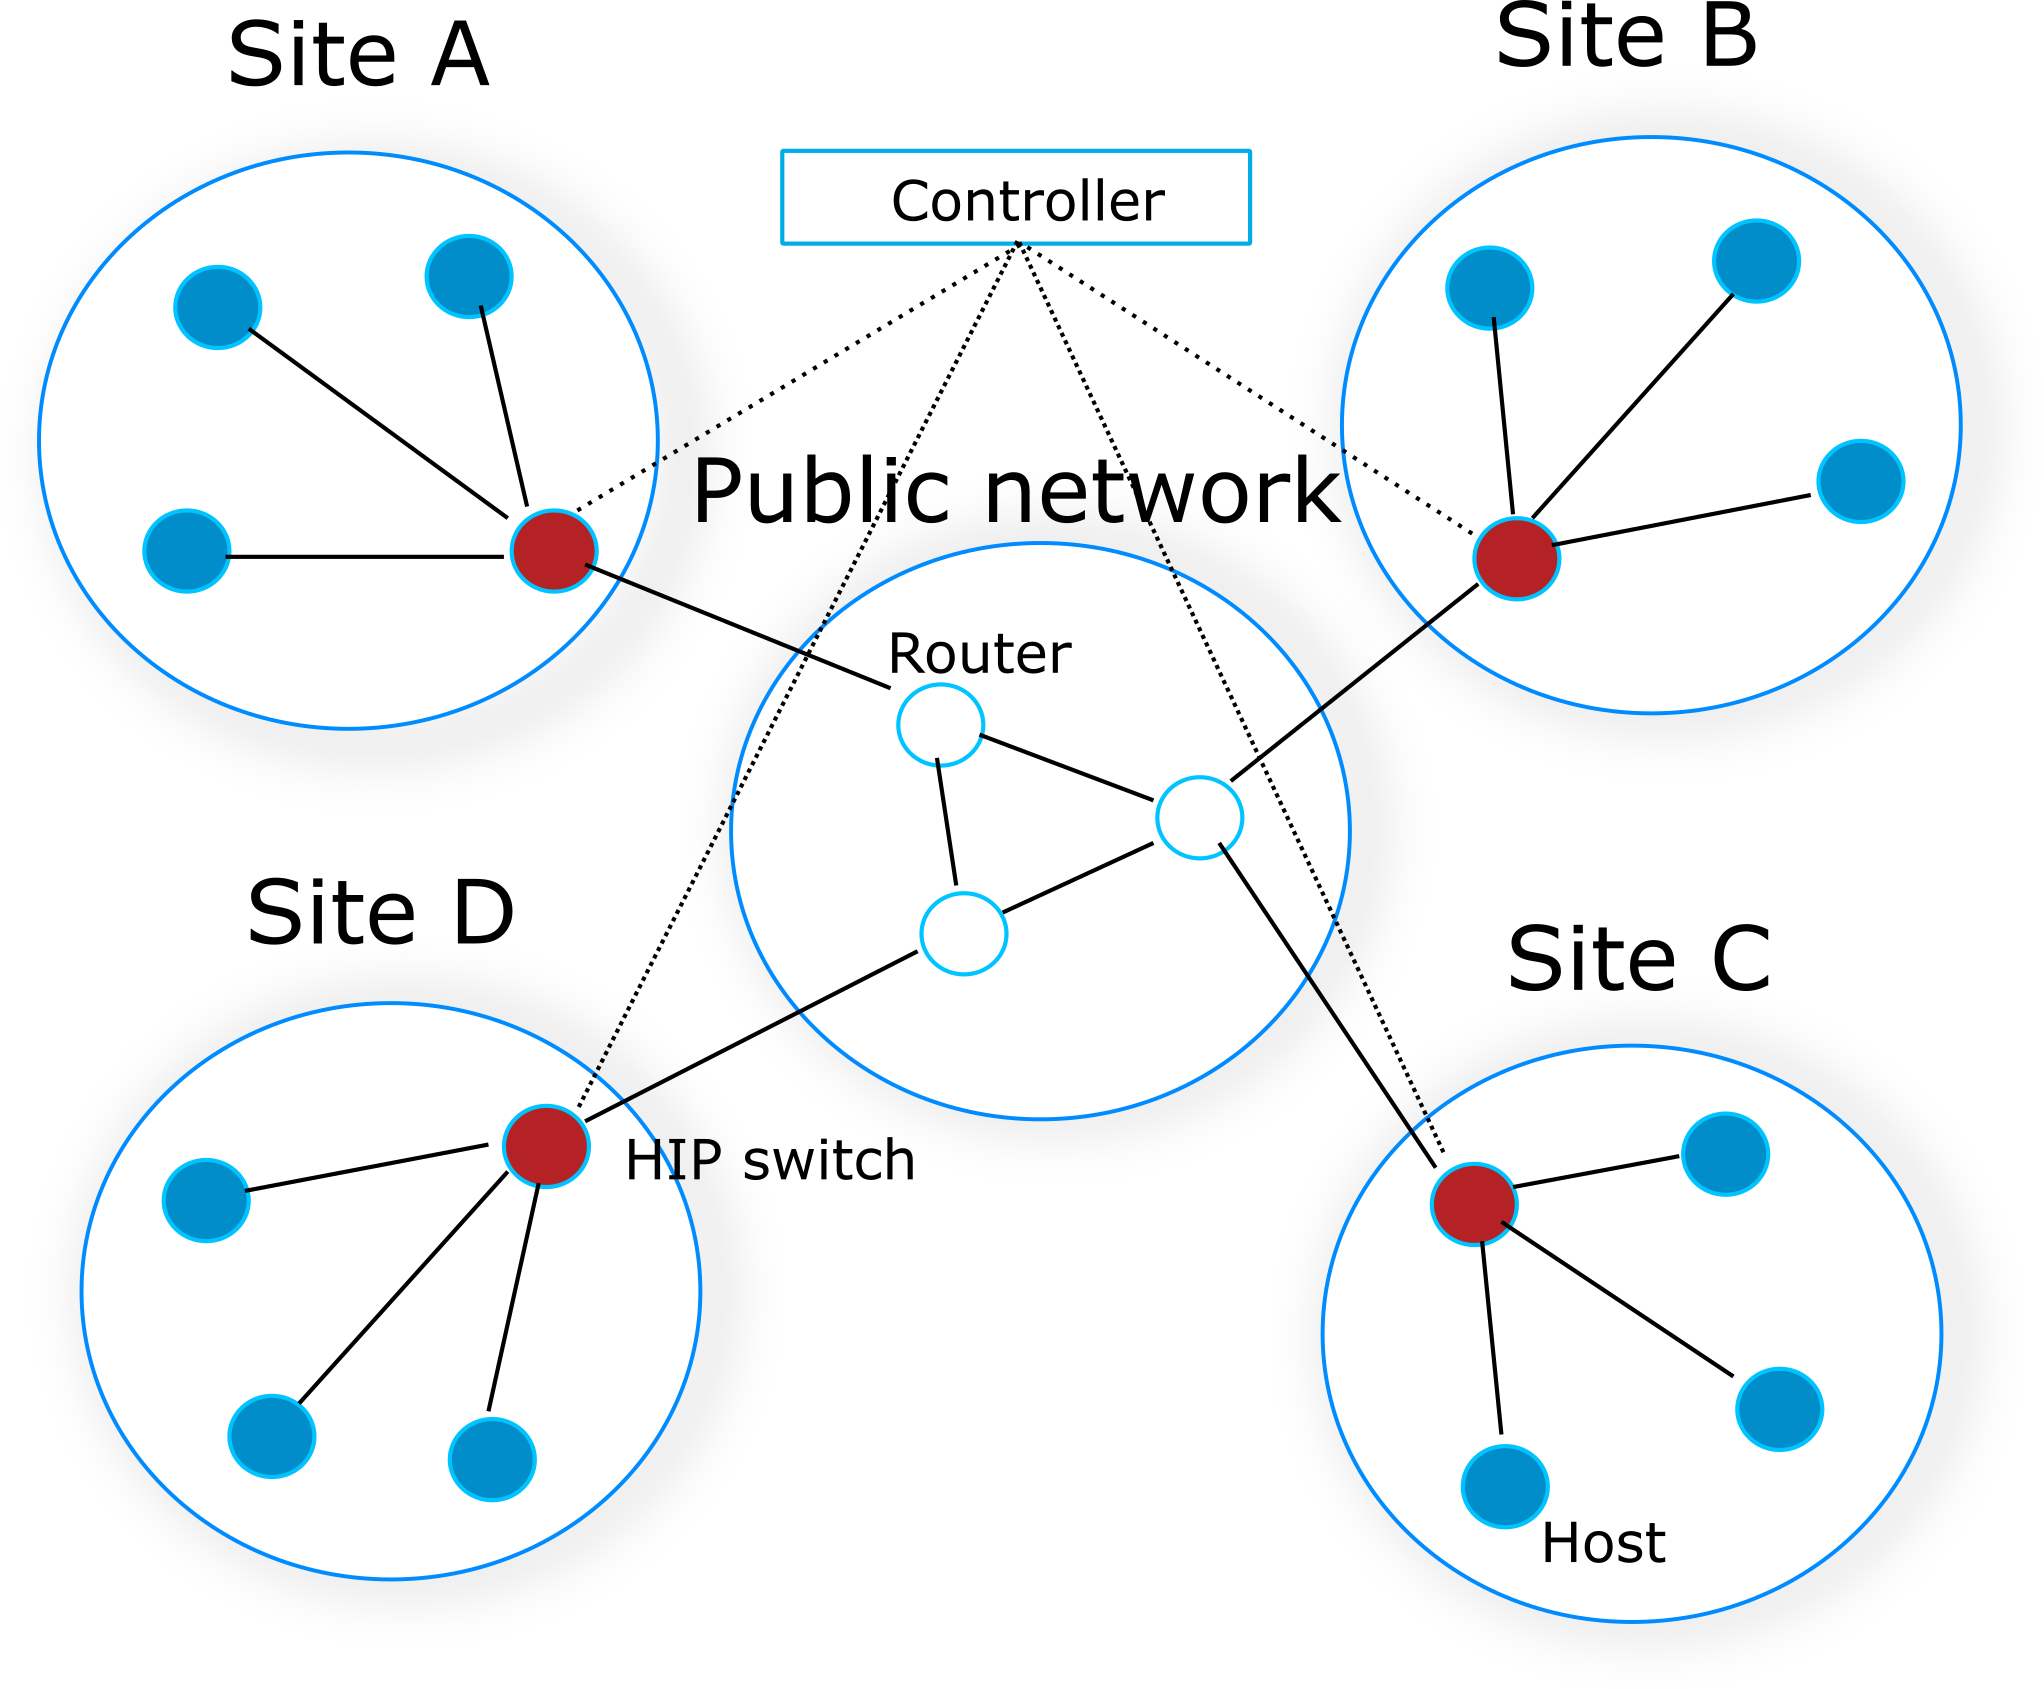
\includegraphics[width=0.7\textwidth]{graphics/hw-hipls.png}
    \caption{HIP-VPLS logical diagram (real hardware deployment)}
    \label{fig:mininet}
\end{figure}

To get a grasp on the performance of HIP-VPLS in the Mininet environment we 
have performed a series of bandwidth tests using {\it iperf} tool. To run
the experiments we have used the UTM emulator (installed on MacBook M1) 
with Ubuntu 22.04 installed. All in all the results were the following: 
the $95\%$ confidence interval for sample mean throughput was 
$58.9 \pm 0.52$ Mbit/s.

We now turn our attention to the real-life deployment 
of HIP-VPLS~\cite{hipvpls-hw, hipvpls-controller}. The system architecture is similar to our Minent prototype
(except that there was a lesser number of HIP switches) shown in Figure~\ref{fig:mininet}. 
Apart from the HIP-VPLS switches, we have also implemented a unique 
control-plane protocol on top of the SSL protocol for communication 
with the central controller on the Internet.

In our deployment, we have used the following setup. For HIP switches we 
have used the dual-network Intel N95 computing platform. We have used $8$ 
port SNR switch to connect $3$ HIP switches, that way we have mimicked the 
IP overlay in the setup. HIP switches had two interfaces: one was facing 
LAN network, the other one was facing the WAN network. 

The microcomputers for HIP switches had the following characteristics: they had $8$GB of RAM memory, 
quad-core Intel N95 CPU (with support for AES and SHA2 NI instructions), $256$ GB of 
solid state hard drive. To wire the routers we have used SNR switches 
(each switch had $8$ $1$ Gbit/s ports and two Small Form Factor (SFP) slots). 
The testbed configuration is shown on Figure~\ref{fig:testbed}.

In the testbed, we had a multihomed server (with one IP facing 
the public network so that HIP switches will be able to connect to 
the controller in the Internet, and one IP in the private range; this server
was playing the role of HIP controller), several legacy microcomputers, 
IP camera, and DHCP and DNS servers.

In our testbed the central controller was responsible 
reporting the liveness of HIP switches as well as provisioning 
the devices with the mesh configuration information, firewall rules 
and MAC-based ACL. For that purpose, we developed a simple 
secure protocol which was utilizing TLS. For example, consider 
the Figure~\ref{devices} which shows the HIP switch registration
and status information.

\begin{figure}[h!]
    \centering
    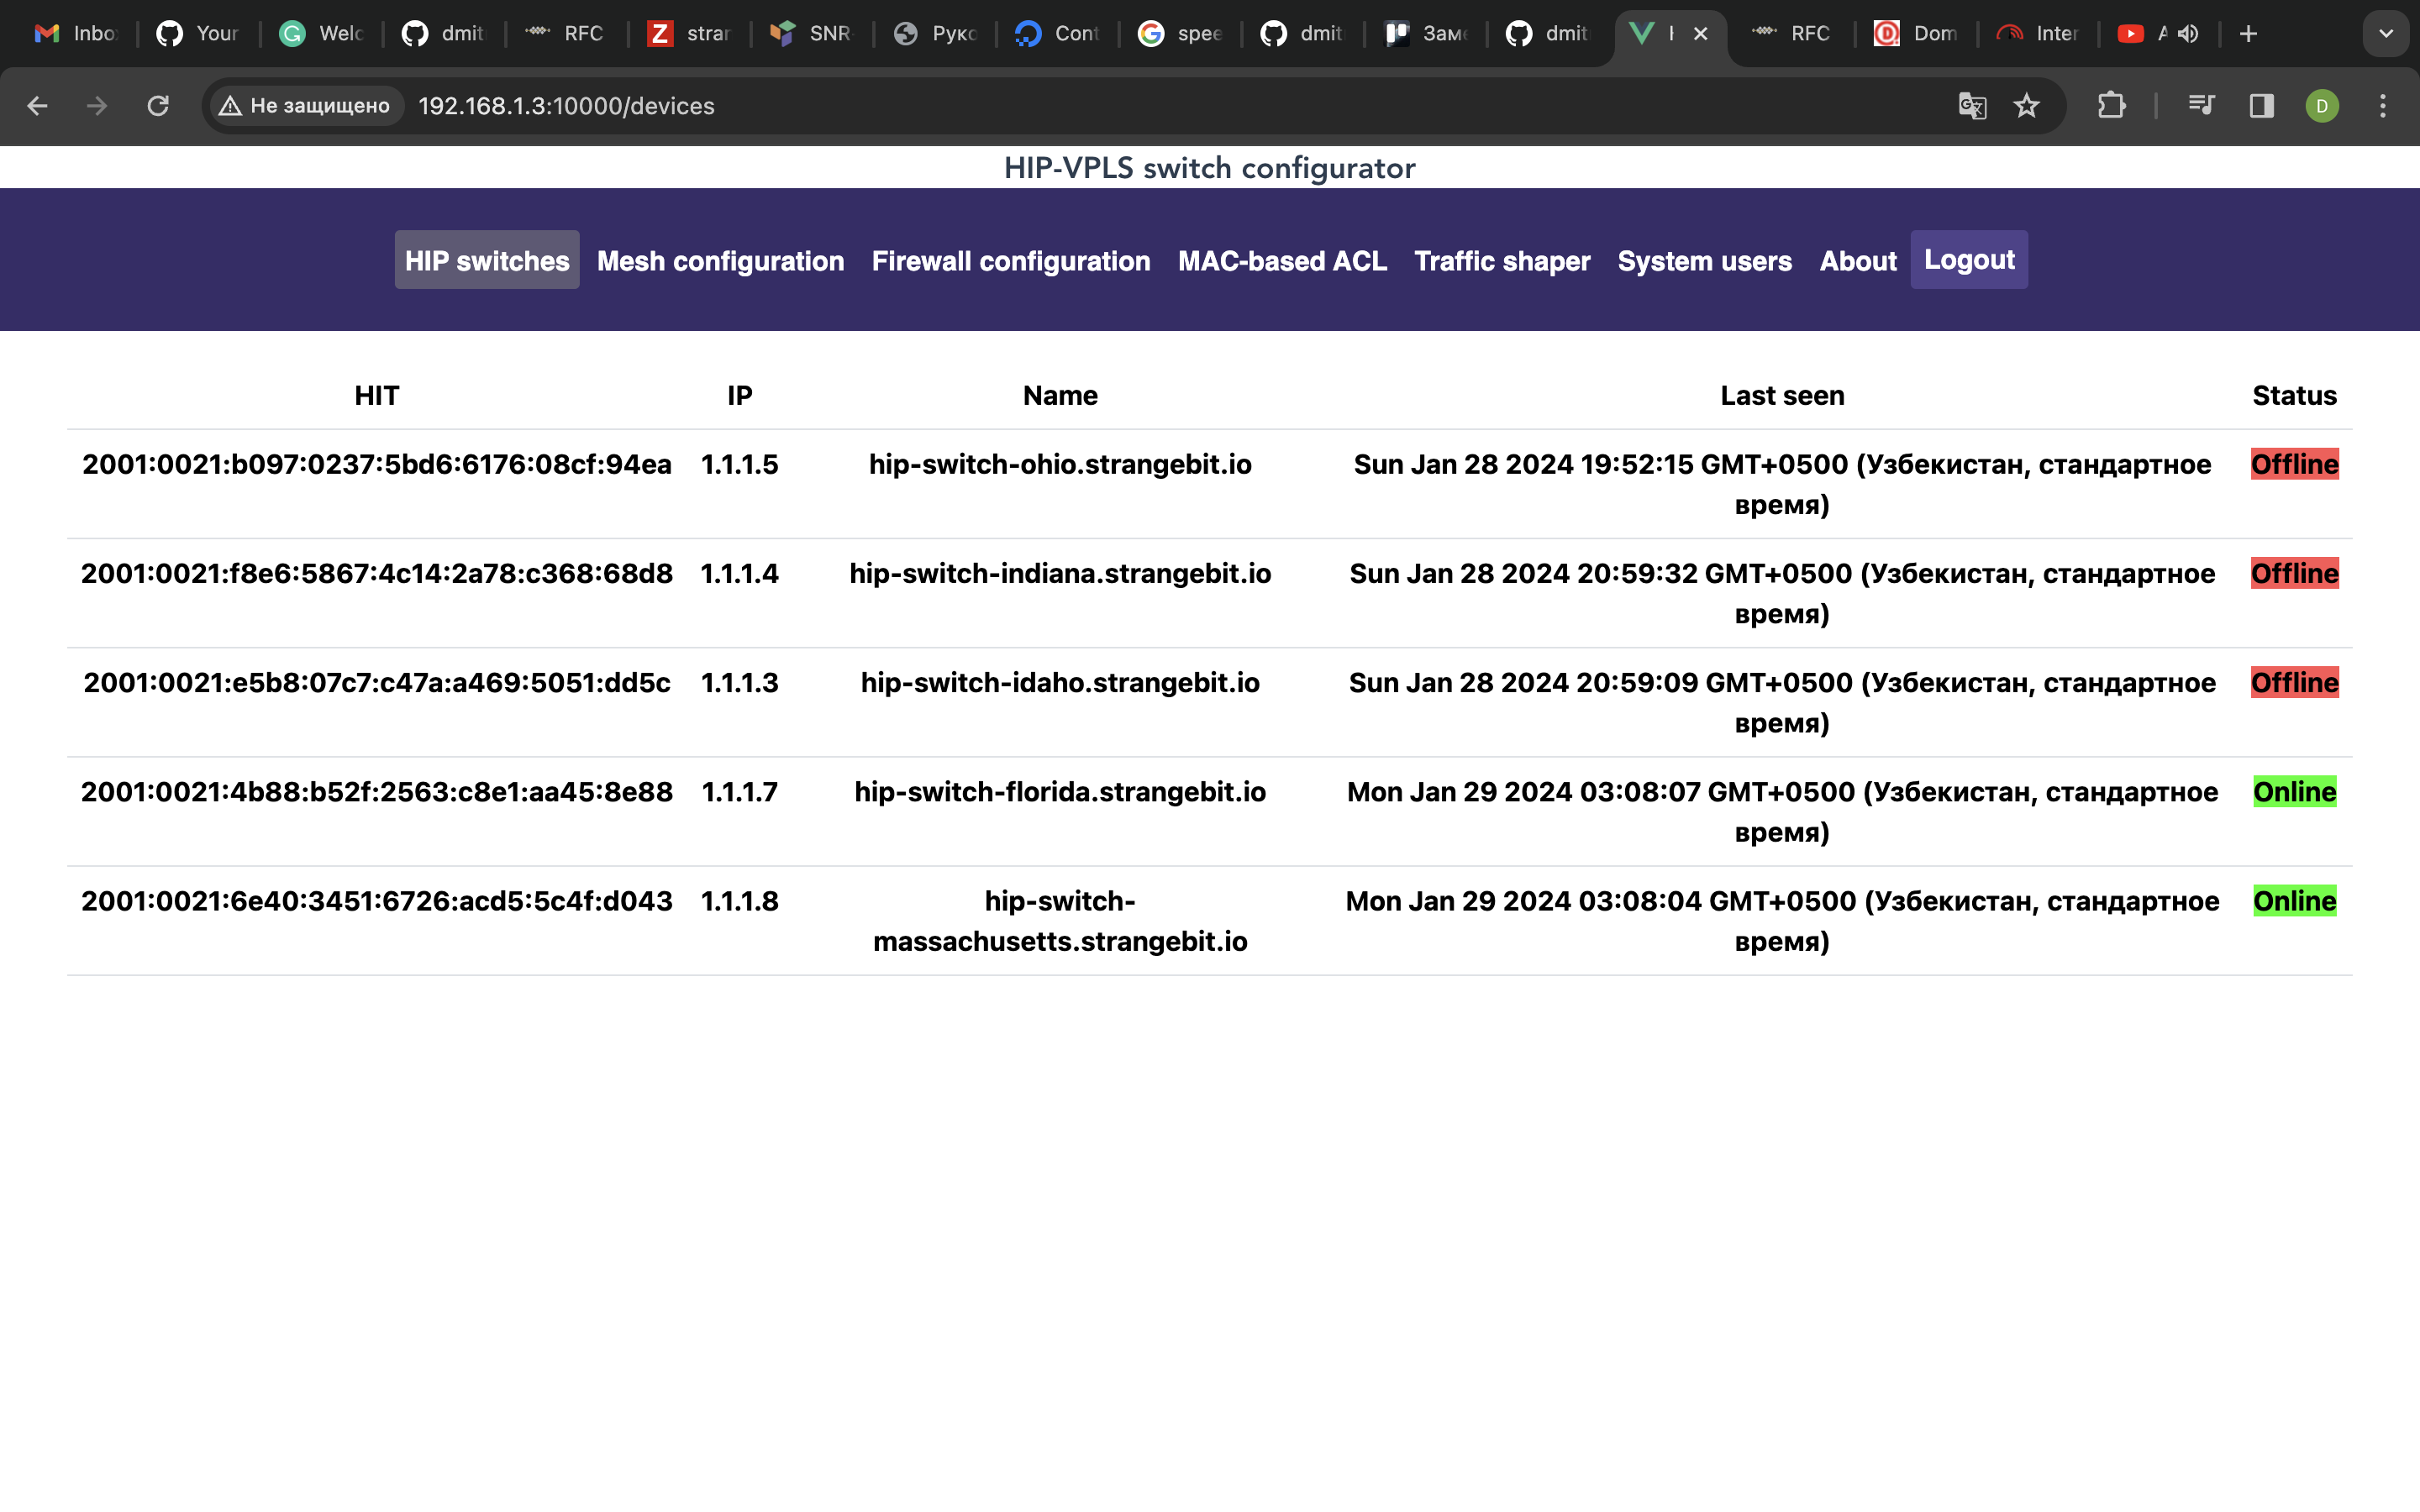
\includegraphics[width=1\textwidth]{graphics/devices.png}
    \caption{HIP-VPLS central controller UI}
    \label{devices}
\end{figure}

According to the protocol, on the one hand, every HIP-VPLS 
the switch was reporting to the central controller (all requests were authenticated 
using the HMAC algorithm together with the shared symmetric 
master secret). In the implementation, switches were reporting 
their presence every $5$ seconds. On the other hand, every HIP-VPLS switch was obtaining 
the configuration from the central controller (such as mesh 
configuration, HIT resolver information, firewall rules, and 
MAC-based ACL). 

\begin{figure}[!ht]
    \centering
    \includegraphics[width=0.9\textwidth]{graphics/testbed.png}
    \caption{Testbed}
    \label{fig:testbed}
\end{figure}

To conclude we have performed a series of real-life experiments to measure the 
performance of the HIP-VPLS network. In Table~\ref{tab:vpls-performance} we show
sample statistics for upload and download throughput. In addition, we have also
measured latency. To perform the measurements we have used {\bf speedtest}
Python library. Thus, on one side, we have connected the MacBook to the HIP switch via a regular
switch. On the other side, we have connected the other HIP switch to a network 
that had connectivity to the Internet. We then performed $100$ rounds of measurements,
collected throughput and latency data and processed the cleaned data using Python
{\it statistics} library. 

\begin{table}
    \centering
    \begin{tabular}{|c|c|c|c|}
    \hline
    Statistics     & Upload (Mbit/s)        & Download (Mbit/s)     & Latency (ms) \\\hline
    Sample mean    & $46.1$                  & $48.2$                 & $5.0$         \\
    Sample std     & $7.1$                   & $2.3$                  & $0.19$        \\
    Sample median  & $44.8$                  & $48.8$                 & $4.9$         \\
    Sample min     & $14.3$                  & $40.0$                 & $4.6$         \\
    Sample max     & $61.3$                  & $50.4$                 & $5.4$         \\
    \hline
    \end{tabular}
    \caption{Performance of HIP-VPLS on Intel N95 CPU}  
    \label{tab:vpls-performance}
\end{table}

\section{Scalable multipoint to multipoint VPN using HIP protocol}

The major problem with the HIP-VPLS is the number of HIP switches and
full-mesh connectivity between these switches. Imagine that there are 
not 10s, but 1000s sites, and that all sites need to be 
combined into a single network. First of all, there will be 
$O(n^2)$ pseudo-wires: for $1000$ PEs there will be  
around $1$M of routing table entries. Second, HIP-VPLS provides 
a single broadcast domain. And so there is going to be 
chaos in the network which will be overwhelmed with broadcast
and multicast Ethernet frames. All these aspects make this type of
arrangement of network unacceptable in the aforementioned scenarios.
Instead, what if we let each site live in its own broadcast
domain, \ie have a separate network address, and combine through 
a series of overlay routers, which will be responsible for 
forwarding the packets between the networks (sites) based on 
inner IPv4 addresses. 

To make the network scalable and reduce the number of pseudowires
we let some nodes play the hub role, that is they will be the backbone 
of the overlay network. While some nodes will be the spoke nodes
and will be connected directly to the sites. It is the hierarchy 
that makes the network scalable. 

It is logical to ask why would someone need to build the multipoint to 
multipoint L3-VPN? Well, hub-and-spoke architecture adds reliability 
to the system: if one node will fail, the entire network will not.
It is, therefore, suggested to build the hub-and-spoke type of L3-VPN
if high dependability of an overlay is a must.

It is worth to look at the overall architecture which we have implemented in
Mininet framework~\cite{hip-l3vpn}. The logical diagram is shown in Figure~\ref{fig:l3vpn}. 
As we have already mentioned, the architecture of the distributed 
L3-VPN network is of hub-and-spoke type. Hub nodes comprise the backbone of the network, whereas,
multiple spoke PE elements are attached to the hubs. 

The security of the network is achieved by using Host Identity Protocol (on a hop-by-hop basis) to negotiate
the authentication and encryption keys, whereas, the actual packet authentication
and encryption is performed on hop-by-hop bases using HMAC-SHA256
and AES (with 256 bits key) algorithms. In our prototype implementation we 
have populated the routing tables manually, however, in practice this 
process should be automated using for example central controller. 

\begin{figure}[!ht]
    \centering
    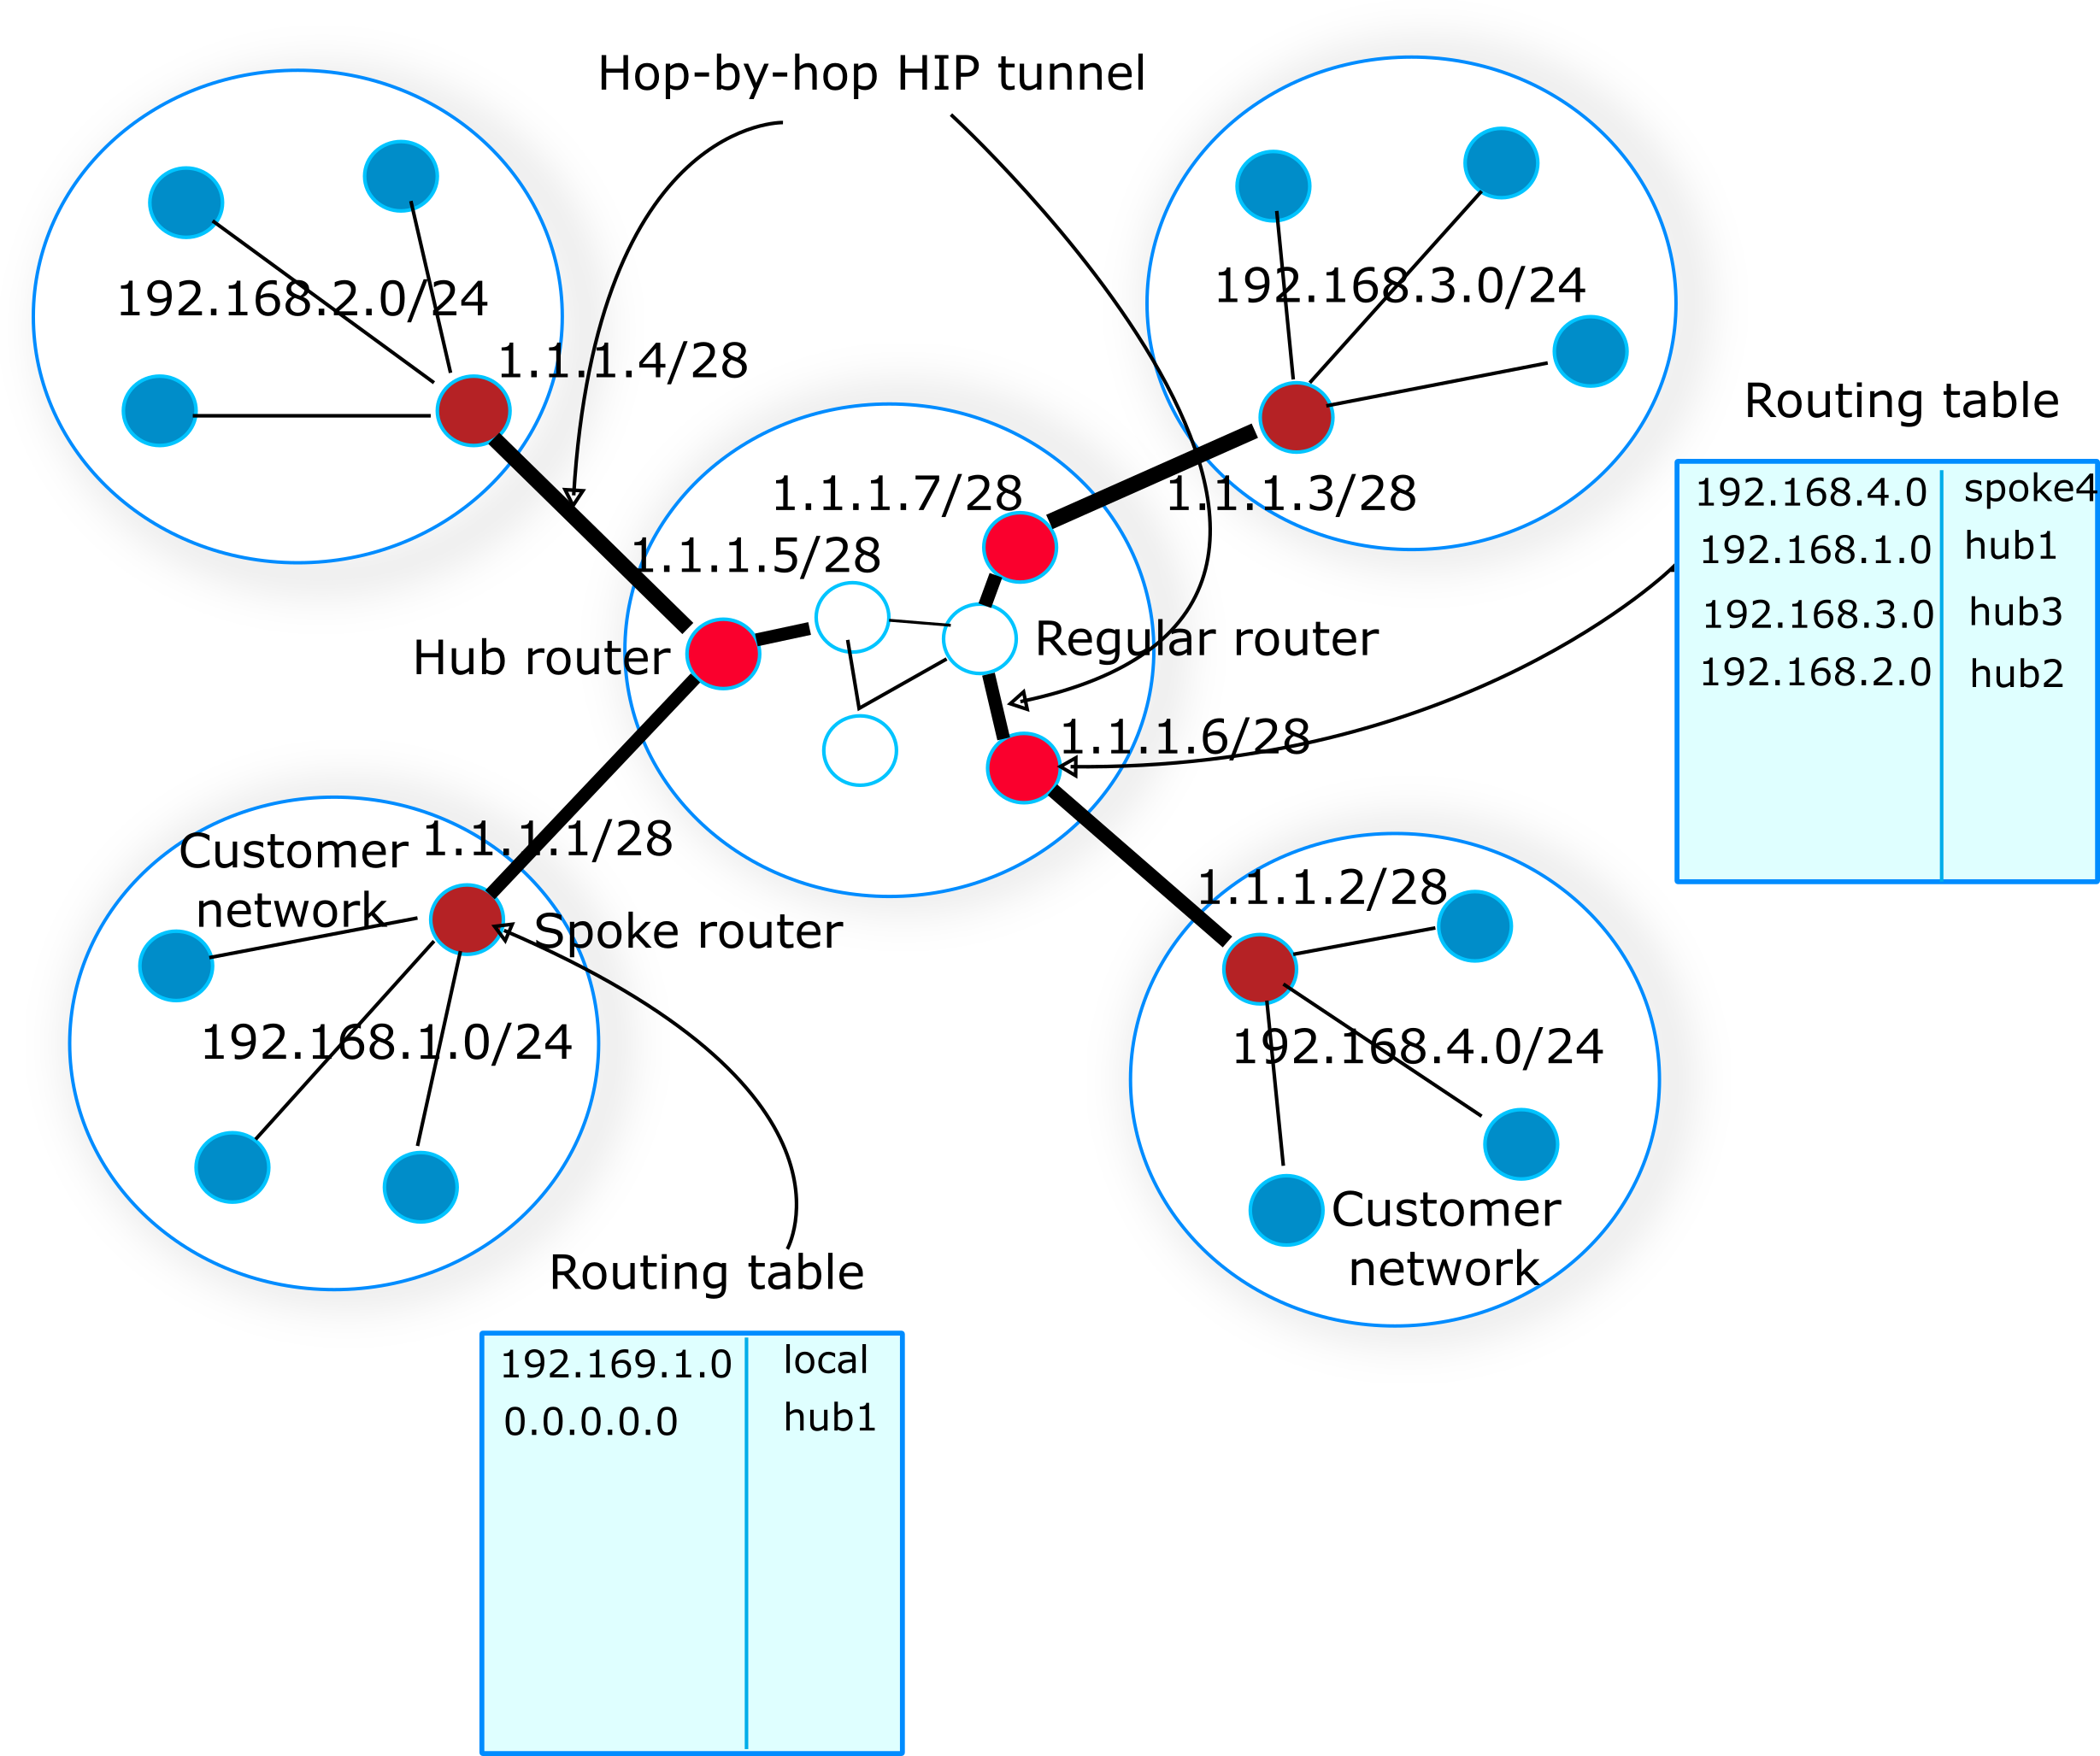
\includegraphics[width=0.9\textwidth]{graphics/l3-vpn.png}
    \caption{HIP-based L3-VPN in Mininet}
    \label{fig:l3vpn}
\end{figure}

To get the taste of the performance of this setup we have performed 
several rounds of experiments with the {\it iperf} utility and measured
the throughput with encryption/authentication enabled. The results 
are the following: $19.7 \pm 0.06$ Mbit/s. This was expected, since the packet
is decrypted and encrypted, as well as HMAC is recalcutated at every hop on 
the path from source CE to destination CE. Perphas, hop-by-hop encryption and authenication can
be done selectively with global secret key so that better performance can be achived.

\section{Comparison of various solutions}

\begin{table}
    \small
    \begin{tabular}{|l|c|c|c|}
    \hline
    Characteristic $\downarrow$ \ Overlay type $\rightarrow$ & L2-VPLS & L3-VPN & HIP-VPLS \\\hline
    Size of forwarding/routing table & $O(n)$ & $O(m)$ & $O(n)$\\\hline
    Number of links in mesh & $O(k^2)$ & $O(k^2)$ & $O(l^2)$ \\\hline
    Privacy (exposure of information) & MACs & IPs & No \\\hline
    Encryption and authentication & Hop-by-hop & Hop-by-hop & PE-to-PE \\\hline
    Tunneling mode & Ethernet-in-IP & IP-in-IP & Ethernet-in-IP \\\hline
    Loop free-topology & 802.1D/Controller & Controller & Not required \\\hline
    \end{tabular}
    \caption {Comparison study of different multipoint VPLS/VPN designs}
    \label{analysis}
\end{table}

In what follows, we compare now different approaches and identify their
characteristics and limitations. In Table~\ref{analysis} we 
compare three different approaches for building overlays with Host 
Identity Protocol. The first one is scalable L2-VPLS with hub-and-spoke
architecture. The second one, L3-VPN, also with hub-and-spoke 
design. And finally, we have HIP-VPLS at our disposal with full mesh connectivity 
of provider equipment (PE).

The first characteristic is the size of the forwarding table on the PE elements. For 
L2-VPLS and L3-VPN it is equal to $O(n)$, where $n$ is the number of regular hosts in the
network. This is obvious, as the MAC address table at least on the edge needs to know
the mapping for each and every host in the network (consider when all hosts talk to 
all other hosts). For L3-VPN the size is considerably smaller since the routing table
contains only IP prefixes of the networks and so equals to $O(m)$, where $m$ is the number 
of sites, hence, the size of the network address prefixes. The reader should understand
that $n \gg m$.

The second important characteristic is the number of links in a mesh network. For L2-VPLS 
and L3-VPN it is equal to $O(k^2)$, where $k$ is the number of hub PEs. For HIP-VPLS
this metric is equal to $O(l^2)$, such that $l$ is the overall number of sites or PEs.
Clearly, $l \gg k$, and hence the L3-VPN achieves better scalability.

What about privacy? Well in scalable L2-VPLS and L3-VPN the MAC and IPs are exposed to intermediate hubs 
(at the end these addresses are used for forwarding). And so if a hub gets compromised 
this information will be leaked to the adversary. In turn, in HIP-VPLS there are no intermediate nodes
in the network since the pseudowires are created end-to-end, and so there is no risk that the 
customer will expose sensitive information to intermediate nodes. Also, in scalable L2-VPLS and scalable L3-VPN 
the encryption and authentication is done in a hop-by-hop manner; whereas, in HIP-VPLS the 
encryption is PE-to-PE (or site-to-site). 

One last important point is the avoidance of loops in the network. For L2-VPLS loop-free topology
is achieved with 802.1D protocol (PE should implement this functionality, because they perform forwarding
tasks) or an SDN central controller. In L3-VPN the loops are avoided with the help of the IP TTL field. 
Also, in L3-VPN the routing tables are constructed centrally and no routing loops will exist 
in the topology. HIP-VPLS archives loop-free topology by assuming that customer networks run an 
instance of STP protocol. There is no need to implement 802.1D STP protocol for HIP switches
since they do not forward Ethernet frames (received from public interface) to all, 
but private interface.

\chapter{Conclusions}

We started this work with the background material on cryptography. Here we covered
established approaches (building blocks) of modern security protocols. In addition, we 
have introduced to the reader more recent developments, such as the LWE encryption scheme.
We see that integration of LWE encryption and signature algorithm into HIP protocol 
can be future work. We then discussed how to build various secure tunnels, \eg with 
SSL, IPSec, and SSH protocols. We covered briefly QinQ tunneling and MPLS protocol.

In the results section, we covered the results for various cryptographic libraries,
including the library which uses Intel NI instructions designed to boost the AES and 
HMAC. We concluded that the Python library with C-bindings is not enough for the 
production setup, and suggested implementing the HIP-VPLS in Rust or C language.
We then moved to the desciption of scalable L3-VPN and HIP-VPLS solutions. We concluded 
the work with a comparison of various characteristics of scalable L2-VPLS, L3-VPN and 
HIP-VPLS solution. 


